\documentclass[12pt, paper=a4]{article}
\usepackage[utf8]{inputenc}
\usepackage[german]{babel}
\usepackage{mathrsfs}
\usepackage{amsmath}
\usepackage{amssymb}
\usepackage{listings}
\usepackage{graphicx}
\usepackage{fancyhdr}

\setlength{\parindent}{0pt}

\author{Mareike G\"ottsch, 6695217, Gruppe 2\\Paul H\"olzen, 6673477, Gruppe 1\\Sven Schmidt, 6217064, Gruppe 1}

\title{FGI 2 Hausaufgaben 9}

\rhead{M. G\"ottsch, G-2; P. H\"olzen, G-1; S. Schmidt, G-1}
\pagestyle{fancy}
\begin{document}
\maketitle
\section*{9.3}

\subsection*{1.}
\subsection*{2.}
Als \"Uberdeckungsgraph zu \(N_{9.3}\) f\"ur die Anfangsmarkierung \(m_0=(2,1,0)^t\) ergibt sich:
\begin{figure}[h!]
	\centering
	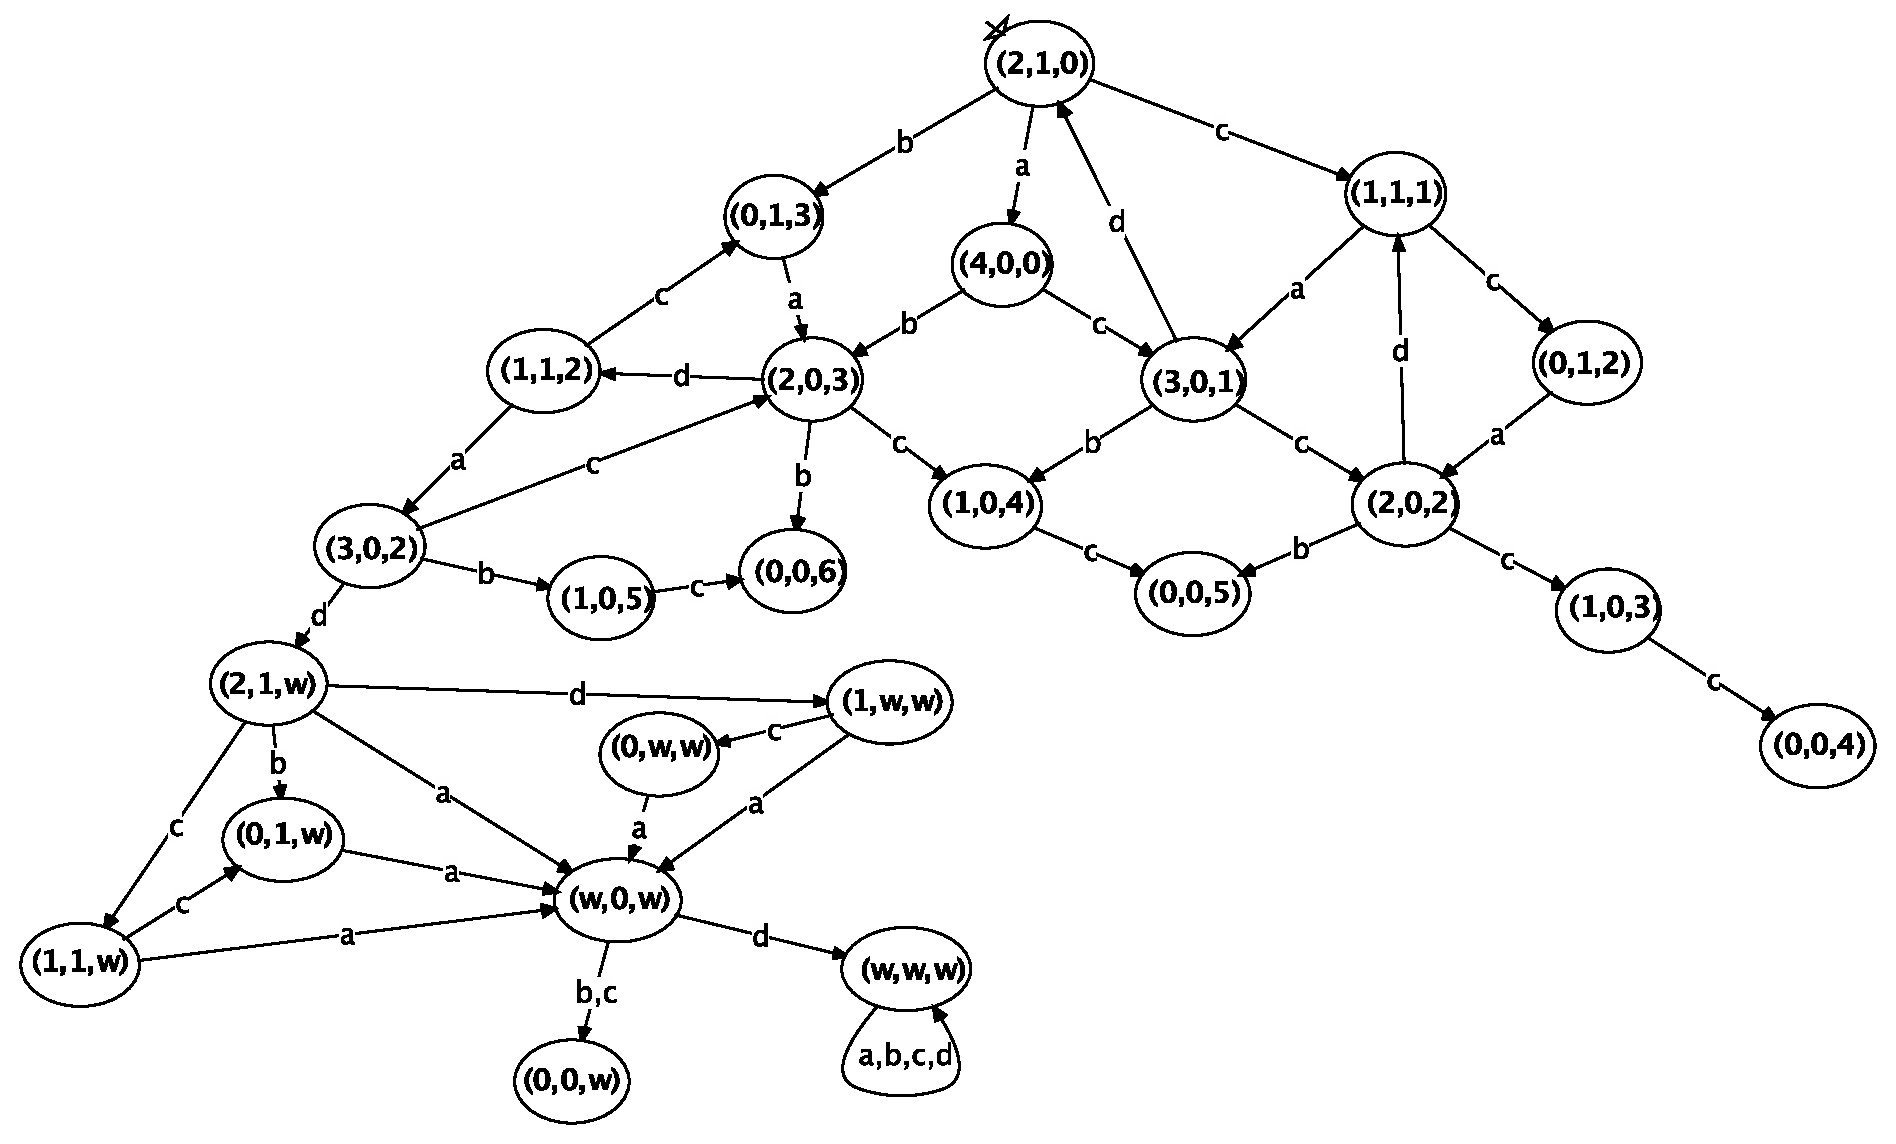
\includegraphics[scale=0.35]{9_3_2.pdf}
	\caption{\"Uberdeckungsgraph von \(N_{9.3}\)}
\end{figure}

\subsection*{3.}


\section*{Aufgabe 9.4}

\section*{Aufgabe 9.5}
	\begin{itemize}
	\item In einem Workflow-Netz sind Quelle a und Senke e beliebig zu w\"ahlen.\\
		Wahr oder falsch?\\
		\textit{(Lesestoff Woche 9, Teil 1)}
	\item Eine Transition kann sowohl einen Uplink als auch (mehrere) Downlinks haben.\\
		Wahr oder falsch?\\
		\textit{(Lesestoff Woche 9, Teil 2)}
	\end{itemize}
\end{document}
